\chapter[La Nebulosa de Orión]{La Nebulosa de Orión: La Fotoevaporación de Discos Protoplanetarios como una Forma de Feedback Estelar}
\thispagestyle{empty}
\label{chap:ONC}
\section{Características Generales}
\begin{figure*}
  \centering
 % \begin{tabular}{cc}
    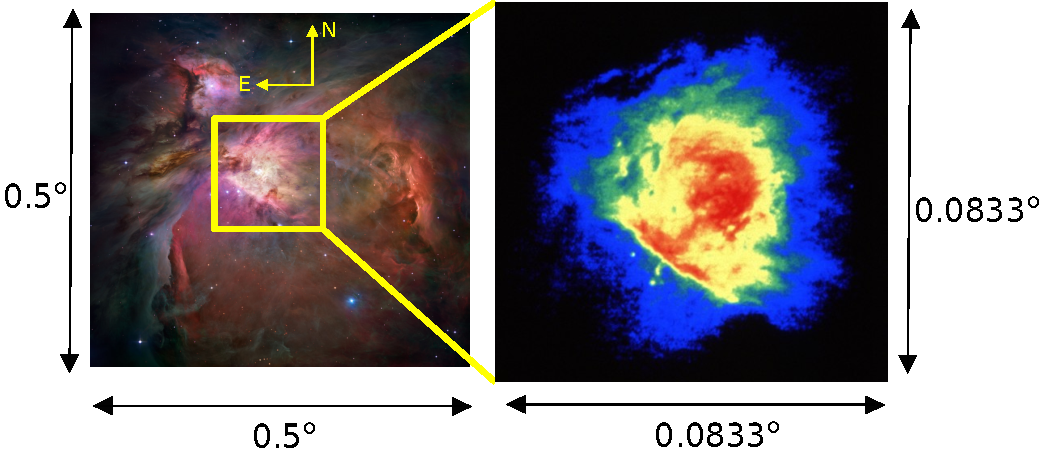
\includegraphics[width=\linewidth]{./Figures/orion-HST-NRAO} 
 % \end{tabular}
    \caption[La Nebulosa de Orión]{Izquierda: La nebulosa de Orion tomada con el Telescopio Espacial Hubble (hubblesite.org). Derecha: La Nebulosa de Orión observada por el VLA en la banda L ($\lambda = \SI{20}{cm}$, $\nu = \SI{1.4}{GHz}$, \citet{Yusef:1990}). La región observada en esta imagen corresponde aproximadamente al recuadro mostrado en la imagen de la izquierda. Créditos: NASA, ESA, NRAO.}
    \label{fig:orion-pretty}
\end{figure*}

El cúmulo de las Nebulosa de Orión (ONC por sus siglas en inglés, figura \ref{fig:orion-pretty}), ubicada a $\sim \SI{414}{pc}$ \citep{Menten:2007}, es probablemente la región \Ion{H}{II} mejor estudiada del cielo (ver apéndice \ref{app:HII}). Forma parte de la nube molecular gigante de Orión, de donde se distinguen dos sub-unidades, llamadas Orión A y Orión B. ONC forma parte de Orión A. El cúmulo de estrellas masivas que se formó y que es responsable de la región \Ion{H}{II} se conoce como asociación OB Ori Id, cuyos miembros más prominentes son un grupo de cuatro estrellas conocidas como el ``Trapecio''. La más masiva de éstas es \thC{}, de clasificación espectral O6 aproximadamente (ver tabla \ref{tab:ionizing-radiation}), tiene una luminosidad de \SI{4e5}{L_\odot} y una temperatura de \SI{4e4}{K}. Cuando la región \Ion{H}{II} se encuentra embebida en el gas molecular, no puede ser visible en el rango óptico del espectro. En el caso de ONC, que se ubica cerca del borde de la nube molecular Orion A, el gas ionizado caliente, que posee una presión mayor que el gas molecular frío, se escapa hacia el gas adyacente de la nube molecular en forma de ``flujo de champaña'', de modo que el gas ionizado se acerca a nosotros a una velocidad de $\sim \SI{3}{km.s^{-1}}$, mientras que ONC se aleja a una velocidad de $\sim \SI{10}{km.s^{-1}}$ (\citet{Stahler:2004}, ver figura \ref{fig:champagne}). De esta manera el gas ionizado puede ser visible por medio de diferentes líneas espectrales, tanto de hidrógeno como de otros elementos. 

\begin{figure}
  \centering
  \begin{tabular}{lr}
    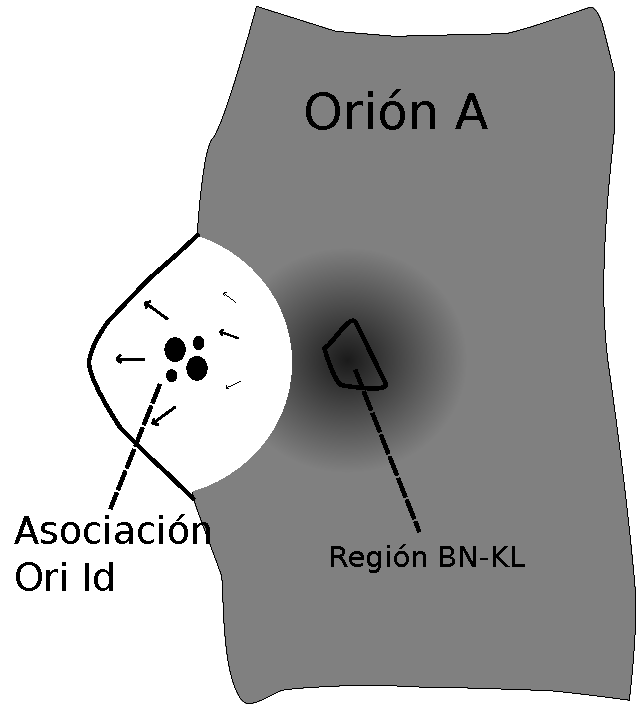
\includegraphics[width=0.4\linewidth]{./Figures/champagne} &
    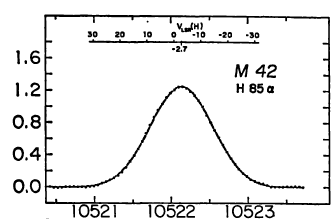
\includegraphics[width=0.5\linewidth]{./Figures/H85-alpha}
    \end{tabular}
  \caption[Asociación Ori Id]{Izquierda: Representación esquemática de la Asociación Ori Id y su ubicación dentro de la nube molecular gigante Orión A. La región BN-KL es una región de formación estelar muy activa donde se observan entre otras cosas, máseres de agua, SiO y flujos moleculares \citep{Stahler:2004}. Derecha: Línea espectral \Ion{H85}{\alpha} de hidrógeno de ONC. El eje horizontal corresponde a la frecuencia en MHz, mientras que el eje vertical representa la temperatura de antena. El espectro muestra un corrimiento al azul que muesta que el gas se acerca a una velocidad de $\sim \SI{3}{km.s^{-1}}$ \citep{Stahler:2004, Churchwell:1970}}
  \label{fig:champagne}
\end{figure}

\section{Proplyds}
\subsection{Descubrimiento}
Observaciones en óptico de la región del Trapecio en filtros de banda angosta de diferentes líneas de emisión tales como \Ion{H}{\alpha}, \Ion{H}{\beta}, [\Ion{O}{III}], [\Ion{N}{II}], [\Ion{S}{II}] y continuo, revelaron la existencia de objetos puntuales visibles notablemente en líneas de alta ionización (\Ion{H}{\alpha}, \Ion{H}{\beta} y [\Ion{O}{III}]) que fueron inicialmente denominados como ``condensaciones nebulares'' \citep{Laques:1979}. Hasta ese momento no se sabía con certeza si esas ``condensaciones nebulares'' eran en realidad condensaciones nebulares (regiones donde la densidad de la nebulosa es inusualmente alta o bien esferas de gas molecular cuya envolvente fue ionizada y que la radiación de la estrella central la está ``erosionando'') o si se trataba de protoestrellas de baja masa cuyo disco protoplanetario estaba siendo fotoevaporado por la estrella central \citep{churchwell:1987}. No fue sino hasta que se contó con observaciones de alta resolución con el Telescopio Espacial Hubble (HST) que se se pudo determinar la verdadera naturaleza de estos objetos \citep{ODell:1993} y la razón por la que se les denominó ``proplyds'' (PROtoPLanetarY DiskS). A su vez se encontraron por primera vez arcos delgados y otras estructuras de gran interés.

\subsection{¿Qué es un proplyd? Breve introducción \citep{Johnstone:1998}}
\label{sec:prop-Johnstone}

Las imágenes del HST de la Nebulosa de Orión mostraron imágenes de discos alrededor de estrellas jóvenes de baja masa. Algunos se ven como siluetas oscuras que contrastan con la nebulosa, y otros casos son visibles en líneas de emisión de líneas de alta ionización. Un proplyd típico tiene forma cometaria, con una cabeza brillante que apunta hacia la fuente de radiación ionizante, y una cola que se extiende en dirección contraria a ésta, (ver figura \ref{fig:prop-shape}). La explicación a esta forma es que se trata de estrellas T-Tauri que quedaron embebidas por la región \Ion{H}{II} en expansión y el disco protoplanetario está siendo fotoevaporado por la radiación ionizante de una estrella masiva (\thC{} en caso de la Nebulosa de Orión), la cabeza es un frente de ionización cuyo radio escala como $R_{\mathrm{IF}} \propto D^{2/3}$, donde $D$ es la distancia a la estrella masiva. La forma de la cola se debe a radiación  difusa, producto de dispersión por polvo y por recombinaciones. \citet{churchwell:1987} ya había notado que la tasa de pérdida de masa observada en el gas ionizado implicaba que la fuente de este gas debía oscurecer a la protoestrella huésped, a menos que proviniera de un disco circunestelar. De la emisión de radio observada, se estima que la densidad electrónica máxima en el IF es de $n_e \sim \SI{e6}{cm^{-3}}$ y la tasa de pérdida de masa es de $\dot{M} \sim \SI{e-7}{M_\odot.yr^{-1}}$.

\begin{figure}
  \centering
  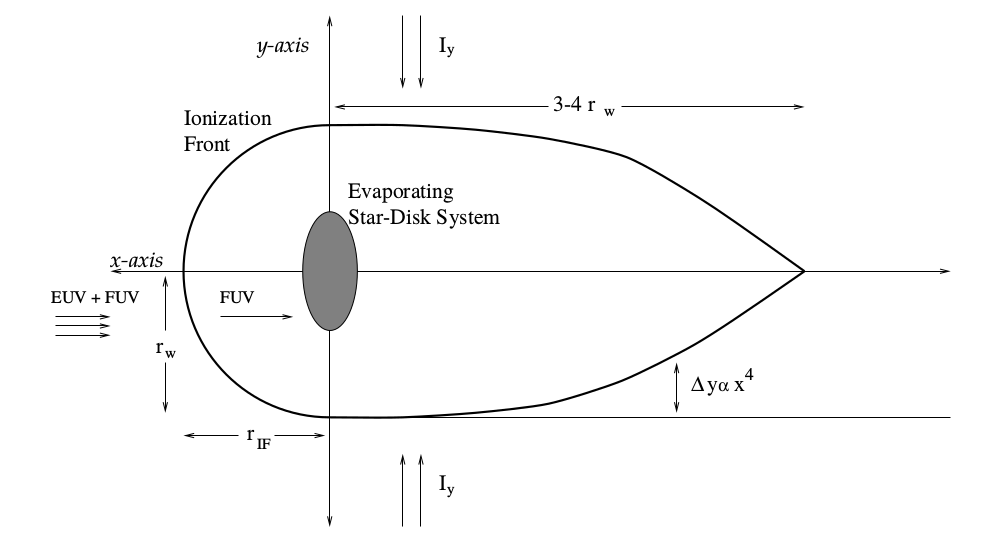
\includegraphics[width=0.8\linewidth]{./Figures/Johnstone-shape}
  \caption[Representación esquemática de un proplyd]{Representación esquemática de la formación de un frente de ionización hemisférico y de una cola de gas fotoevaporado detrás del disco en proceso de fotoevaporación \citep{Johnstone:1998}. La línea gruesa exterior representa la interfaz donde existe equilibrio entre ionizaciones y recombinaciones en el flujo fotoevaporado. $r_{\mathrm{IF}}$ y $r_w$ representan el radio del frente de ionización en las direcciones de los ejes $x$ e $y$, respectivamente. $I_y$ representa el campo de radiación difusa. Por detrás del disco, la radiación difusa calienta el gas del disco provocando otro flujo fotoevaporado. $\Delta y$ es la diferencia entre la forma actual del frente de ionización por detrás del disco y una forma cilíndrica, y determina la forma de la cola. En esta interfaz debe de haber balance entre ionizaciones provocadas por el flujo $F_y \simeq \pi I_y$ y recombinaciones en el flujo fotoevaporado, y como la densidad de este flujo disminuye al alejarse del disco a lo largo del eje $x$, entonces la zona donde se da el equilibrio de ionización ocurre cada vez más cerca del eje $x$. \citet{Johnstone:1998} muestra que la forma de la cola es tal que $\Delta y \propto x^4$, donde $x$ es la distancia al disco a lo largo del eje $x$. Por otro lado, también se muestra que la cola termina cuando $\Delta y = r_w$ y esta condición se da cuando $x \sim 3 r_w$.} %como que el flujo de radiación $I_y$ es capaz de penetrar más cerca del eje $x$ conforme uno se aleja del disco, donde el flujo fotoevaporado es menos denso.}
    \label{fig:prop-shape}
\end{figure}


\subsection{Mecanismos de fotoevaporación \citep{Johnstone:1998}}
\label{sec:photoevaporation}

El principal mecanismo de fotoevaporación es el campo de radiación de la estrella central, en la parte ultravioleta del espectro electromagnético. Según la masa de la estrella central, podemos tener dos clases de flujo radiativo: Dominado por el ultravioleta lejano (FUV, $h\nu < \SI{13.6}{eV}$) o dominado por el ultravioleta extremo (EUV, $h\nu \geq \SI{13.6}{eV}$). En general, el FUV se encarga de disociar moléculas y de calentar el gas de la región de fotodisociación (PDR) hasta temperaturas de \SI{100}{} - \SI{1000}{K}, mientras que el EUV puede ionizar el gas y elevar su temperatura hasta \SI{e4}{K}. El EUV no puede atravesar el frente de ionización (IF) pero el FUV sí. Inicialmente la forma del disco impone una geometría cilíndrica en el flujo fotoevaporado, pero eventualmente los gradientes de presión tornan esta geometría en esférica, como se muestra en la figura \ref{fig:flux-geometry}.

\begin{figure}
  \centering
  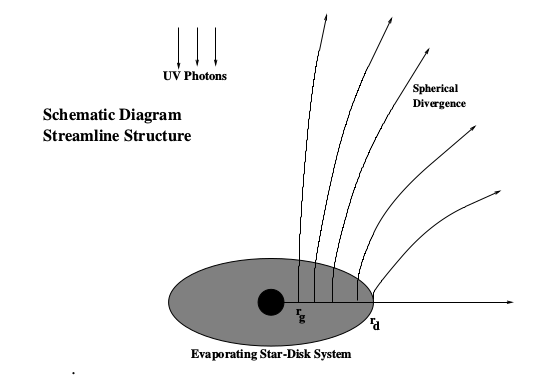
\includegraphics[width=0.7\linewidth]{./Figures/Johnstone-1}
  \caption[Geometría del flujo fotoevaporado]{Geometría del flujo fotoevaporado de un disco protoplanetario de radio $r_d$ bajo un flujo de fotones ultravioleta provenientes de una fuente puntual lejana. Inicialmente el disco impone una geometría cilíndrica para el flujo, pero los gradientes de presíon en el ambiente convierten rápidamente la geometría del flujo en esférica. El gas que se encuentra a distancias menores a $r_g$ de la estrella central (ecuación \ref{eq:grav-radius}) es retenido por la gravedad de ésta \citep{Johnstone:1998}.}
  \label{fig:flux-geometry}
\end{figure}

En el caso de que el flujo sea dominado por el EUV, la presión térmica del flujo fotoevaporado es determinada por la fotoionización, la PDR producida por el FUV es delgada. El gas calentado por el FUV se mueve de manera subsónica ($v_I \propto r^{-2}$) hasta llegar al IF, donde alcanza una velocidad de \SI{0.5}{km.s^{-1}} y la tasa de pérdida de masa depende de la tasa de ionización inducida por el EUV.

Si el flujo está dominado por el FUV, la presión térmica depende del calentamiento por el FUV. El gas tibio se expande como un viento que empuja el IF lejos del disco que alcanza velocidades supersónicas, pero luego atraviesa un choque isotérmico que lo desacelera y llega al frente de ionizacion a \SI{0.5}{km.s^{-1}}. La tasa de pérdida de masa la determina la temperatura de la PDR, el flujo FUV y la opacidad del polvo a las longitudes de onda del FUV. Este caso y el anterior se muestran en la figura \ref{fig:EUV-FUV-IF}.

Las ecuaciones de continuidad de la masa y el momento restringen la velocidad del flujo neutro antes de alcanzar el IF. Mas allá de éste, la presión del gas hace que éste se expanda a velocidades del orden de una a dos veces la velocidad del sonido, que es de $c_{\mathrm{I}} \sim \SI{3}{km.s^{-1}}$ para el gas neutro, y de $c_{\mathrm{II}} \sim \SI{10}{km.s^{-1}}$ para el gas ionizado. Para el gas neutro dentro del IF hay dos posibles soluciones: si el gas neutro es supersónico entonces el IF será de baja densidad (Tipo R) con bajo contraste de densidad entre gas neutro y gas ionizado. O si el gas neutro es subsónico se formará un IF tipo D con un gran contraste de densidad entre el gas neutro y el gas ionizado. Sin embargo, ya mostramos que sin importar qué tipo de radiación domina la fotoevaporación, el gas neutro permanece a velocidades subsónicas al llegar al IF (figura \ref{fig:EUV-FUV-IF}), por lo que dicho frente será tipo D.

\begin{figure}
  \centering
    \begin{tabular}{cc}
      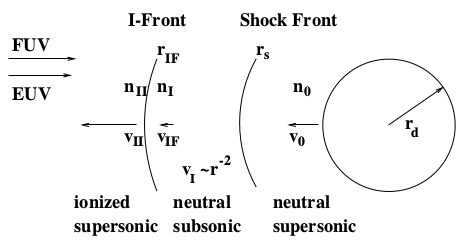
\includegraphics[width=0.5\linewidth]{./Figures/Johnstone-2} &
      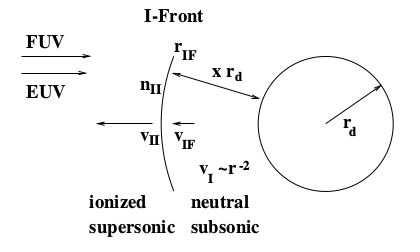
\includegraphics[width=0.5\linewidth]{./Figures/Johnstone-3}
    \end{tabular}
    \caption[Representación esquemática del flujo fotoevaporado]{Representación esquemática de las regiones del flujo fotoevaporado de un proplyd. Izquierda: Cuando el flujo es dominado por el FUV, se acelera a velocidades supersónicas pero atraviesa un choque isotérmico que lo desacelera a velociades subsónicas. Derecha: Flujo dominado por EUV, que llega a velocidades subsónicas al frente de ionización \citep{Johnstone:1998}.}
    \label{fig:EUV-FUV-IF}
  \end{figure}
  
  
Sin importar el tipo de mecanismo de fotoevaporación dominante, el flujo fotoevaporado existe solo si la presión térmica supera a la gravedad de la protoestrella. Entonces, el flujo fotoevaporado solo existe a partir de un radio crítico $r_g$, donde este radio se estima a partir del balance entre la energía necesaria para escapar de una órbita kepleriana y la energía térmica:
\begin{align}
  r_g = \frac{GM_*}{c^2} \label{eq:grav-radius}
\end{align}
Donde $M_*$ es la masa de la protoestrella y $c$ es la velocidad del sonido del gas. Para las protoestrellas típicas del Trapecio la masa típica es de
$M_* = \SI{0.2}{M_\odot}$. Utilizando las velocidades del sonido para el gas neutro e ionizado, encontramos que el radio gravitacional para un flujo dominado por el EUV es de $r_{\mathrm{gII}} \sim \SI{2}{AU}$ y para un flujo dominado por el FUV es de $r_{\mathrm{gI}} \sim \SI{20}{AU}$.
